\documentclass[tikz]{standalone}
\usepackage{amsmath,amssymb,amsfonts}
\usepackage{pgfplots}

\pgfplotsset{compat = newest}

\begin{document}
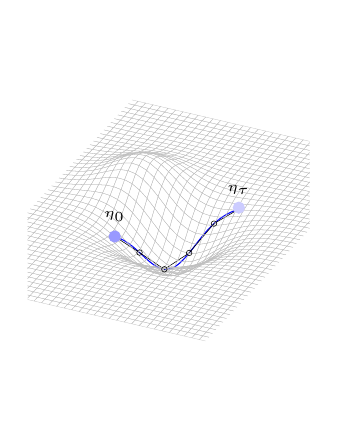
\begin{tikzpicture}[font=\small]
  \begin{axis}[
    unit vector ratio*=1 1 1,
    hide axis = true,
    xmin = -1.5,
    xmax = 1.5,
    zmin = -2.5,
    zmax = 2.5
    ]    
    \addplot3+[
    mesh,domain=0:1,samples=50,samples y=0,no markers,
    colormap={}{
      color(0cm)=(blue) color(1cm)=(blue)
    },
    ](
    {2.3*x-1},
    {2.3*x-1},
    {-1.5*exp(-2*(2.3*x-1)^2)+1.0*exp(-0.75*((2.3*x+0.2)^2+(2.3*x-2.2)^2))}
    );
    \addplot3+[
    mesh,domain=0:1,samples=6,samples y=0,mark=o,
    very thin,mark size=1pt,draw=black,
    ](
    {2.3*x-1},
    {2.3*x-1},
    {-1.5*exp(-2*(2.3*x-1)^2)+1.0*exp(-0.75*((2.3*x+0.2)^2+(2.3*x-2.2)^2))}
    );
    \addplot3 [
    mesh, 
    draw = lightgray,
    line width = 0.1pt,
    samples = 50]
    {-1.5*exp(-0.5*(x^2+y^2))+1.0*exp(-0.75*((x+1.2)^2+(y-1.2)^2))};
    \addplot3[blue!40, only marks] coordinates{(-1,-1,-0.177)};
    \addplot3[blue!20, only marks] coordinates{(1.3,1.3,0)};
    \draw[minimum size=6cm] (-1, -1, 0.4) node {\tiny $\eta_0$};
    \draw[minimum size=6cm] (1.3, 1.3, 0.5) node {\tiny $\eta_\tau$};
  \end{axis}
\end{tikzpicture}
\end{document}
